\chapter{Model implementation}
\label{ch:model-implementation}

This chapter discusses the implementation of the 
aforementioned models. We firstly introduce the 
Python framework used in the implementation and go 
over the preprocessing steps that were used. 
Then we will look at each model separately and discuss the implementation 
of these models as well as the optimization of the hyperparameters.

The implementation of the models and the testing is done in Python. 
The source code can be found on 
GitHub\footnote{\url{https://github.com/pavelzw/GEFCom14-S-comparison}}.

\section{pyWATTS}
\label{sec:pywatts}

In order to combine the models in a joint environment 
and reuse steps like the calculation of the pinball loss, 
it makes sense to use some kind of pipeline structure for the code. 
\Textcite{Heidrich2021} introduced 
pyWATTS\footnote{\url{https://github.com/KIT-IAI/pyWATTS}}, a framework 
for creating pipelines for time series forecasting. 

\begin{figure}[h]%
    \centering
    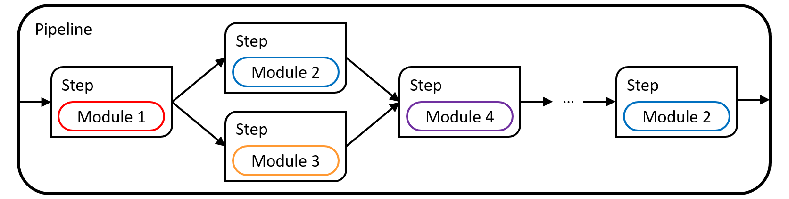
\includegraphics[width=0.9\textwidth]{plots/pywatts-schematic.pdf}
    \caption[pywATTS schematic]{pyWATTS schematic from \Textcite{Heidrich2021}. 
    Each step of the algorithm can be added in a single pipeline module. 
    A module can be used multiple times like for training and forecasting purposes.}
    \label{fig:pywatts-schematic}%
\end{figure}

pyWATTS can create different stages for each subtask of a pipeline like 
data pre- and postprocessing, model training, model testing and 
rendering predictions into images, a schematic of the pipeline 
can be found in Figure \ref{fig:pywatts-schematic}. Wrappers for scikit-learn 
modules are already implemented so the creation of a pipeline 
for scikit-learn models is relatively straightforward. 
For other neural network models, one can simply create a class that inherit the 
\texttt{BaseWrapper} class. The \texttt{fit}- and \texttt{transform}-methods 
need to be implemented to train the model and make predictions with it. 
Simple transformations like for example the NNQF preprocessing step can be 
wrapped by a \texttt{FunctionModule} and inserted into the pipeline.
For each stage in the pipeline, one can output the data of the model 
with callbacks like the \texttt{CSVCallback} to save \texttt{csv}-files or 
the \texttt{ImagePlotCallback} to save images.

\section{Data Preprocessing}
\label{sec:data-preprocessing}

From all predictors in Table \ref{table:predictors}, only SSRD, STRD, TSR, TP and TCC are used 
because they are the most relevant predictors: SSRD, STRD and TSR can model the hypothetical maximum power 
output while TCC is relevant because it correlates with how much sun light actually reaches the solar stations. 
Total precipitation is also important in the winter months since the solar stations can be covered with snow and no sun light gets through.
Since the Variables SSRD, STRD and TSR are all provided as accumulated fields, they first need to be decumulated.
This can be done by subtracting the previous value from the current value for each day: 
\[ \tilde{x}_i = \begin{cases}
    x_i - x_{i-1}, &i \mod 24 \neq 0, \\
    x_i, &\text{otherwise}.
\end{cases} \]
Figure \ref{fig:strd-accumulated-vs-decumulated} shows both the accumulated and decumulated fields. 
A machine learning algorithm works better with the decumulated field since the decumulated field directly correlates 
with the power output of the solar plant.

Since machine learning models often work better with normalized data, it makes sense to normalize the predictors 
so that they take values in \([0,1]\) instead of \([0,\infty)\). We can do that by dividing every value by the maximum of the values. 

\begin{figure}[h]%
    \centering
    \subfloat[\centering STRD accumulated]{{\includegraphics[width=7cm]{plots/strd_accumulated.pdf} }}%
    \qquad
    \subfloat[\centering STRD decumulated]{{\includegraphics[width=7cm]{plots/strd_decumulated.pdf} }}%
    \caption[STRD accumulated vs. decumulated]{STRD accumulated vs. decumulated. 
    In order to get the actual data, we first need to subtract the previous point \(x_{t-1}\) from \(x_t\).}%
    \label{fig:strd-accumulated-vs-decumulated}%
\end{figure}

\section{Hyperparameter Tuning}

Since all models share a similar environment, 
hyperparameter optimization can be performed in a similar manner for every model.
They are tuned using the 
hyperopt package by \Textcite{Bergstra2013}\footnote{\url{https://github.com/hyperopt/hyperopt}}.

In order to use it, we need to set up a space of 
all parameters that we want to optimize and 
then call the \texttt{fmin} method to minimize the loss 
calculated by the pyWATTS pipeline. 
The algorithm to select the next set of hyperparameters is 
the Tree-structured Parzen Estimator approach (TPE) 
that is described by \Textcite{Bergstra2011}.

\section{Quantile Regression Forests}
\label{sec:implementation-qrf}

\section{NNQF}
\label{sec:implementation-nnqf}

Since the NNQF method is only a preprocessing step for the target values, 
we still need to decide which model we want to use for fitting the 
conditional distribution function. 
\Textcite{Ordiano2019} tried fitting each of the \(99\) quantiles 
with a polynomial of maximum degree \(1\) to \(4\) or a multi layer perceptron 
with \(6\) or \(10\) hidden neurons. Since the multi layer perceptrons landed 
significantly better results, I will focus on them. 

Because the data is a time series, timepoints that are close are correlated. 
That's why we not only take the predictor value \(x_n \in \R^D\) of time point \(n\) 
but also \(x_{n-1}, \ldots, x_{n-H+1}\) as predictor values, where \(H\) is the number of lags.
All in all, we want to fit a function \(\func{f_q}{\R^{D\times H}}{\R}\), 
where \( f(x_n, \ldots, x_{n-H+1}; \theta_{(q)})\) is the conditional \(q\)-quantile of the target value \(Y_n\).

In order to remove quantile crossing, \Textcite{Ordiano2019} postprocesses the conditional quantiles:
\[ \hat{y}_{(q)} = \begin{cases}
    \max\set{ f(x; \theta_{(q)}), 0 }, &\text{if } q = 0.01, \\
    \max\set{ f(x; \theta_{(q)}), f(x; \theta_{(q-0.01)}) }, &\text{else.}
\end{cases}\]

In this thesis, I used another approach: 
I simply sorted all estimated conditional quantiles \(\set{ f(x; \theta_{(q)}) \;|\; q\in \set{0.01, \ldots, 0.99} }\) 
and set \(\hat{y}_{(q)}\) as the \((q\cdot 100)\)-th entry of the sorted list. This resulted in a significant performance improvement 
in comparison to taking the maximum. \todo{add numbers to show significant improvement!}

\section{Spline Quantile Function RNNs}
\label{sec:implementation-sqf-rnn}

The implementation for the SQF-RNN model is provided by 
\Textcite{Gasthaus2019} on GitHub\footnote{\url{https://github.com/awslabs/gluon-ts}} in the 
Gluon-TS package by \Textcite{Alexandrov2019}.

The key difference between the SQF-RNN model and the DeepAR model from 
\Textcite{Salinas2017} is that the DeepAR implementation uses a 
parametric distribution and optimizes the distribution parameters 
based on the maximum likelihood estimation. 
In the DeepAR default implementation, a Student's \(t\)-distribution is used. 
In the SQF-RNN case, spline quantile functions are used and their parameters 
are optimized based on the CRPS. 
For complex problems, the specification of a probabilistic distribution 
that fits the data is often not trivial. 
As the CRPS is closely related to the pinball loss (see \ref{ch:crps}), 
this helps in the GEFCom14 problem since it directly minimizes the given metric.

The data preprocessing steps are the same as in the QRF case. 
After preprocessing, the training data is converted into a \texttt{ListDataset} and fitted with the 
\texttt{DeepAREstimator} class. The frequency of the model is set to one hour and 
prediction length to 28, 30 or 31 days since the task is to predict one full month. 
In order to use quantile splines with three parts as the output distribution, 
we need to set the distribution output of the model to \texttt{PiecewiseLinearOutput(num\_pieces=3)}, 
i.e., linear spline quantile functions. 
The default implementation of DeepAR does not use the predictors but only uses the previous time data. 
In order to use the predictors \(x_1, \ldots, x_n \in \R^D\), 
we need to change the value of \texttt{use\_feat\_dynamic\_real}
to \texttt{True} or else the model will ignore them. 

After training the model for seven epochs with the data that is available from the previous months, 
we need to predict the upcoming month. This is done by calling the \texttt{predict()} 
method from the predictor that we got after training.
Then, the quantiles are calculated from the results and used to 
calculate the pinball loss.

In order to get better and more consistent results, 
seven independent models are trained simultaneously and in the predicition step the average of all models is used as output.

Because the DeepAR model is similar to a recurrent neural network, 
the tunable hyperparameters also look similar. 
The context length, e.g., the number of steps to unroll the RNN 
before computing predictions, the number of RNN layers as well as the number of RNN cells 
can be tuned for each layer. 
The cell type of the RNN can be either an LSTM or a gated recurrent unit (GRU) cell.
Another hyperparameter is the dropout regularization: 
the dropout rate and the dropout cell type can be tuned 
with available cell types being \texttt{ZoneoutCell}, 
\texttt{RNNZoneoutCell}, \texttt{VariationalDropoutCell} 
and \texttt{VariationalZoneoutCell}.
For the output distribution, the number of spline pieces can be adjusted.
For the training part, the usual hyperparameters like the number of epochs, batch size, 
learning rate, learning rate decay, patience, gradient clip and weight decay can be tuned.
The parameters after tuning and their corresponding optimization spaces 
are shown in Table \ref{table:sqf-rnn-hyperparameters}.
The resulting losses were all in the range \([0.02, 0.025]\) but the best loss 
was already achieved by the default configuration. No noticable performance improvement is visible.

\begin{table}[h!]%
    \caption{SQF-RNN Hyperparameters}
    \label{table:sqf-rnn-hyperparameters}
    \rowcolors{2}{white}{gray!25}
    \centering
    \footnotesize
    \begin{tabular}{lll}
    \toprule \noalign{\smallskip}
    \tableheads Hyperparameter & \tableheads Optimization space & \tableheads Final value \\ 
    \midrule
    Context length          & \set{\(1\) week, 
                              \(1\) month, \(2\) months} & \(1\) month \\
    RNN layers              & \(\set{2, 3, 4}\)          & \(2\) \\
    RNN cells per layer     & \(\set{20, 40, 60, 100}\)  & \(40\) \\
    RNN cell type           & \set{LSTM, GRU}            & LSTM \\
    Dropout rate            & \(\set{0.01, 0.1, 0.5}\)   & \(0.1\) \\
    Dropout Cell Type       & --                         & \texttt{ZoneoutCell} \\
    Number of spline pieces & \(\set{2, 3, 4, 5}\)       & \(3\) \\
    Number of epochs        & --                         & \(7\) \\
    Batch size              & --                         & \(32\) \\
    Learning rate           & \(\set{0.0005, 0.001, 0.01, 
                              0.05, 0.1, 0.2, 0.5}\)     & \(0.001\) \\
    Learning rate decay     & \(\set{0.3, 0.5, 0.7}\)    & \(0.5\) \\
    Patience                & --                         & \(10\) \\
    Gradient clip           & --                         & \(10\) \\
    Weight decay            & --                         & \(10^{-8}\) \\
    Ensemble size           & --                         & \(3\) \\
    \bottomrule
    \end{tabular}
\end{table}